\documentclass[aspectratio=169,10pt]{beamer}

% ── Tema ──────────────────────────────────────────────────────────────────────
\usetheme{Madrid}
\usecolortheme{default}
\usefonttheme{professionalfonts}

% Paleta MendesLobo: azul estrutura + laranja acento
\definecolor{mlblue}{RGB}{18,52,86}
\definecolor{mlorange}{RGB}{214,100,28}
\definecolor{mlgray}{RGB}{240,242,245}
\definecolor{mlgreen}{RGB}{39,120,71}
\definecolor{mlred}{RGB}{180,35,35}
\definecolor{mlpurple}{RGB}{123,94,167}
\definecolor{mlteal}{RGB}{13,122,122}

\setbeamercolor{structure}{fg=mlblue}
\setbeamercolor{frametitle}{bg=mlblue,fg=white}
% Subtítulo do frame destacado em âmbar sobre a barra azul (hierarquia seção/frame)
\definecolor{mlamber}{RGB}{245,166,35}
\setbeamercolor{framesubtitle}{fg=mlamber}
\setbeamerfont{framesubtitle}{size=\footnotesize,series=\bfseries}
\setbeamercolor{title}{bg=mlblue,fg=white}
\setbeamercolor{block title}{bg=mlblue,fg=white}
\setbeamercolor{block body}{bg=mlgray}
\setbeamercolor{alerted text}{fg=mlorange}
\setbeamercolor{example text}{fg=mlgreen}
\setbeamertemplate{navigation symbols}{}

% ── Pacotes (apenas os disponíveis nesta instalação texlive) ───────────────────
\usepackage[utf8]{inputenc}
\usepackage[T1]{fontenc}
\usepackage[provide=*,portuguese]{babel}
\usepackage{amsmath,amssymb}
\usepackage{tabularx}
\usepackage{array}
\usepackage{graphicx}
\usepackage{xcolor}
\usepackage{tikz}
\usetikzlibrary{arrows.meta,positioning,shapes.geometric,fit,backgrounds,calc,shadows}

% ── Comandos utilitários ───────────────────────────────────────────────────────
\newcommand{\yes}{\textcolor{mlgreen}{$\checkmark$}}
\newcommand{\no}{\textcolor{mlred}{---}}
\newcommand{\half}{\textcolor{mlorange}{$\circ$}}
\newcommand{\role}[1]{\texttt{\small #1}}
\newcommand{\tool}[1]{\texttt{\footnotesize #1}}
\newcommand{\arr}{$\rightarrow$}

% ── Numeração em árvore (1 / 1.2 / 2.2.1 / 2.5.2.2) via contadores manuais ─────
% Beamer numera nativamente section.subsection (2 níveis) via \thesection/\thesubsection.
% Para um 3º e 4º nível (2.2.1, 2.5.2.2) não há contador nativo de navegação em beamer,
% então definimos mlc3/mlc4 amarrados ao subsection via [chave], como um \newcounter
% comum de LaTeX --- nenhum pacote externo faz isso "de graça" além do próprio beamer.
\newcounter{mlc3}[subsection]
\newcounter{mlc4}[mlc3]

\makeatletter
\newcommand{\pathnum}{%
  \ifnum\value{mlc4}>0
    \thesection.\thesubsection.\arabic{mlc3}.\arabic{mlc4}%
  \else\ifnum\value{mlc3}>0
    \thesection.\thesubsection.\arabic{mlc3}%
  \else
    \thesection.\thesubsection%
  \fi\fi
}
\makeatother

\newcommand{\lvlA}{\stepcounter{mlc3}}   % entra no 3º nível (ex.: 2.2 -> 2.2.1)
\newcommand{\lvlB}{\stepcounter{mlc4}}   % entra no 4º nível (ex.: 2.5.2 -> 2.5.2.1)

% \mtitle{Texto do título} -- imprime o número da árvore + título no frametitle
% Hierarquia visível em todo frame: seção como título; número da árvore +
% título específico como subtítulo destacado (âmbar) dentro da barra.
\newcommand{\mtitle}[1]{%
  \frametitle{\insertsection}%
  \framesubtitle{\pathnum\;·\; #1}}

% ── Metadados ─────────────────────────────────────────────────────────────────
\title{Agente Engenheiro de Planejamento Sênior\\[4pt]\large Esteira, Catálogo, Papéis \& Fluxos de trabalho}
\subtitle{Mendes Lobo Construção}
\author{Bruno Peixoto}
\date{\today}
\institute{Uso interno --- confidencial}

% ── Início ────────────────────────────────────────────────────────────────────
\begin{document}

% ═══════════════════════════════════════════════════════════════════════════
\begin{frame}[plain]
  \titlepage
\end{frame}

% ═══════════════════════════════════════════════════════════════════════════
\begin{frame}{Agenda}
  % Agenda até o nível X.Y (decisão 15/07) — os subitens 2.2.x/2.4.x/2.5.2.x
  % ficam só no agenda.md (referência completa). Ao mudar seções/frames,
  % atualizar este frame, o agenda.md e as \section/\subsection.
  \begin{columns}[T]
    \column{0.23\textwidth}
    {\small\textbf{\textcolor{mlblue}{1. Preâmbulo}}}\\[4pt]
    {\footnotesize
    1.1. Motivação\\
    1.2. Resumo executivo\\
    1.3. Modelo de interação e\\
    \hspace*{10pt}arquitetura\\
    1.4. Notação simbólica\\}
    \column{0.23\textwidth}
    {\small\textbf{\textcolor{mlorange}{2. Esteira de planejamento}}}\\[4pt]
    {\footnotesize
    2.1. Etapas e entregáveis\\
    2.2. Catálogo\\
    2.3. Cronograma: precedências\\
    \hspace*{10pt}e quantitativos\\
    2.4. Banco de recursos\\
    2.5. Regras de negócio\\
    2.6. Cenários e cubo analítico\\
    2.7. Ciclos de vida e\\
    \hspace*{10pt}rastreabilidade\\}
    \column{0.23\textwidth}
    {\small\textbf{\textcolor{mlpurple}{3. Dinâmica de interação}}}\\[4pt]
    {\footnotesize
    3.1. Papéis de acesso e\\
    \hspace*{10pt}permissões\\
    3.2. Matriz de responsabilidades\\
    3.3. Workflows por papel\\
    3.4. Hand-offs\\[12pt]}
    \column{0.2\textwidth}
    {\small\textbf{\textcolor{mlgreen}{4. Encerramento}}}\\[4pt]
    {\footnotesize
    4.1. Síntese e próximos passos\\[12pt]}
    {\footnotesize\itshape\textcolor{mlgray!40!black}{Apêndice:\\
    A.1. Fluxo de entrega\\
    A.2. Ferramentas MCP por grupo}}
  \end{columns}
\end{frame}

% ═══════════════════════════════════════════════════════════════════════════
\section{Preâmbulo}
% ═══════════════════════════════════════════════════════════════════════════

\subsection{Motivação}
\begin{frame}
  \mtitle{Motivação: a Dor do Orçamento em Planilha}
  \centering
  \begin{minipage}{0.72\textwidth}
    \begin{alertblock}{Hoje --- onde dói}
      \begin{itemize}
        \item Cronograma, equipes e custo em \textbf{silos}: \emph{pool} de
          recursos sistematicamente inexistnte, mob/demob com risco de duplicação
        \item Catálogo atualizado \textbf{sem governança}: quem mudou,
          quando e por quê não ficam registrados
        \item Cenários de decisão \textbf{não auditáveis}: o que mudou entre
          o que-if e a decisão final?
        \item Proposta reaberta meses depois \textbf{não reproduz} o
          número --- preços mudaram por baixo
        \item Decisão comercial com \textbf{uma única configuração}:
          sem what-if de frentes, jornada ou pool
      \end{itemize}
    \end{alertblock}
  \end{minipage}
\end{frame}

\subsection{Resumo executivo}
\begin{frame}
  \mtitle{Resumo Executivo}
  \begin{columns}[T]
    \column{0.48\textwidth}
    \begin{block}{O que entregamos}
      \begin{enumerate}\small
        \item \textbf{Pipeline auditável}, do escopo ao resultado financeiro
        \item \textbf{Versionamento} de planos, catálogo e BDI
        \item \textbf{Regras de custo e BDI} formalizadas e reconciliadas
        \item \textbf{5 papéis} de acesso e regra dos quatro olhos
        \item Entrega de código separada da atualização de dados
        \item Monitoramento fim a fim com testes automáticos
        \item Exploração de cenários para decisão de negócio
      \end{enumerate}
    \end{block}
    \column{0.48\textwidth}
    \begin{block}{Garantias do sistema}
      \begin{itemize}\small
        \item \textbf{Reprodutibilidade}: cada execução é fotografada
        \item \textbf{Auditabilidade}: trilha completa do catálogo ao preço de venda
        \item \textbf{Isolamento}: catálogo novo não quebra projetos existentes
        \item \textbf{Otimização}: cronograma minimiza o prazo por algoritmo de agendamento
        \item \textbf{Rastreabilidade}: quem mudou o quê, quando e por quê
        \item \textbf{Resiliência}: retorno automático e seguro em falhas
      \end{itemize}
    \end{block}
  \end{columns}
\end{frame}

\subsection{Modelo de interação e arquitetura}
\begin{frame}
  \mtitle{Modelo de Interação e Arquitetura}
  \begin{columns}[T]
    \column{0.55\textwidth}
    \centering
    \resizebox{!}{7.1cm}{%
    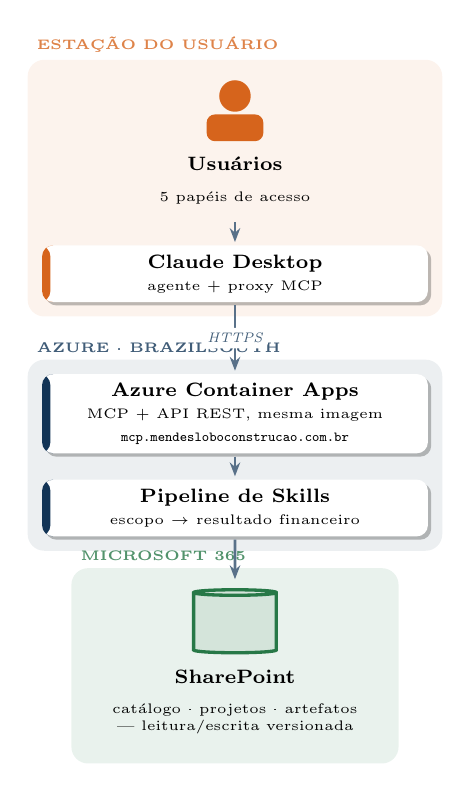
\begin{tikzpicture}[
        % card: fundo branco, sombra suave, barra de acento à esquerda
        cardbase/.style={draw=none,fill=white,rounded corners=4pt,
                    drop shadow={shadow xshift=1.2pt,shadow yshift=-1.2pt,
                                 opacity=0.25,fill=black},
                    minimum width=4.9cm,minimum height=0.72cm,
                    font=\scriptsize,align=center,inner xsep=8pt},
        cardO/.style={cardbase,path picture={\fill[mlorange]
          (path picture bounding box.south west) rectangle
          ([xshift=3pt]path picture bounding box.north west);}},
        cardB/.style={cardbase,path picture={\fill[mlblue]
          (path picture bounding box.south west) rectangle
          ([xshift=3pt]path picture bounding box.north west);}},
        cardG/.style={cardbase,path picture={\fill[mlgreen]
          (path picture bounding box.south west) rectangle
          ([xshift=3pt]path picture bounding box.north west);}},
        zona/.style={rounded corners=6pt,inner sep=5pt},
        arr2/.style={-{Stealth[length=5pt]},mlblue!70,line width=1pt,
                     shorten <=1pt,shorten >=1pt},
        alab/.style={font=\tiny\itshape,text=mlblue!80,fill=white,
                     rounded corners=2pt,inner sep=2pt,midway},
        dbicon/.style={cylinder,draw=mlgreen,fill=mlgreen!20,very thick,
                       shape border rotate=90,aspect=0.3,
                       minimum width=1.05cm,minimum height=0.8cm},
      ]
      % ── ícone de usuário (cabeça + tronco) ──
      \node[circle,fill=mlorange,minimum size=0.4cm] (uhead) {};
      \node[rounded corners=3pt,fill=mlorange,minimum width=0.72cm,
            minimum height=0.34cm,below=0.02cm of uhead] (ubody) {};
      \node[font=\bfseries\scriptsize,below=2pt of ubody] (ulabel) {Usuários};
      \node[font=\tiny,below=0.5pt of ulabel] (usub) {5 papéis de acesso};
      \node[fit=(uhead)(ubody)(ulabel)(usub),inner sep=2pt] (users) {};
      % ── cards ──
      \node[cardO,below=0.32cm of users] (cd)
        {\textbf{Claude Desktop}\\{\tiny agente + proxy MCP}};
      \node[cardB,below=0.9cm of cd,minimum height=0.92cm] (aca)
        {\textbf{Azure Container Apps}\\{\tiny MCP + API REST,
         mesma imagem}\\{\tiny\texttt{mcp.mendesloboconstrucao.com.br}}};
      \node[cardB,below=0.32cm of aca] (pipe)
        {\textbf{Pipeline de Skills}\\{\tiny escopo \arr\ resultado
         financeiro}};
      % ── ícone de banco de dados (cilindro) ──
      \node[dbicon,below=0.65cm of pipe] (spicon) {};
      \node[font=\bfseries\scriptsize,below=2pt of spicon] (splabel) {SharePoint};
      \node[font=\tiny,align=center,below=0.5pt of splabel,
            text width=3.4cm] (spsub) {catálogo · projetos · artefatos ---
            leitura/escrita versionada};
      \node[fit=(spicon)(splabel)(spsub),inner sep=2pt] (sp) {};
      % ── zonas de agrupamento (atrás dos cards) ──
      \begin{scope}[on background layer]
        \node[zona,fill=mlorange!8,fit=(users)(cd),
              label={[font=\tiny\bfseries,text=mlorange!80,anchor=south west,yshift=-1pt]north west:ESTAÇÃO DO USUÁRIO}] {};
        \node[zona,fill=mlblue!8,fit=(aca)(pipe),
              label={[font=\tiny\bfseries,text=mlblue!80,anchor=south west,yshift=-1pt]north west:AZURE · BRAZILSOUTH}] {};
        \node[zona,fill=mlgreen!10,fit=(sp),
              label={[font=\tiny\bfseries,text=mlgreen!80,anchor=south west,yshift=-1pt]north west:MICROSOFT 365}] {};
      \end{scope}
      % ── fluxo ──
      \draw[arr2] (users) -- (cd);
      \draw[arr2] (cd) -- node[alab]{HTTPS} (aca);
      \draw[arr2] (aca) -- (pipe);
      \draw[arr2] (pipe) -- (sp);
    \end{tikzpicture}}
    \column{0.42\textwidth}
    \begin{block}{Princípio}
      \small O usuário fala com o agente, nunca direto com o servidor.
      MCP e API REST compartilham a mesma imagem e a mesma pipeline.
    \end{block}
    \vspace{4pt}
  \end{columns}
\end{frame}

\subsection{Notação}
\begin{frame}
  \mtitle{Notação Simbólica (referência)}
  \scriptsize
  \begin{columns}[T]
    \column{0.48\textwidth}
    \begin{block}{\small Catálogo · produção · preço}
      \begin{tabular}{@{}p{1.5cm}p{4.6cm}@{}}
        $\rho_i$ & produtividade horária de atividade $i$ [un/h] \\
        $\rho^{\text{sin}}_i$ & derivada pelo grafo de sinergia \\
        $\gamma_i,\gamma_r$ & custo horário (equipe, recurso) \\
        $p_i^c, p_i^o$ & preço unitário (catálogo, operacional) \\
        $\tau_i$ & razão $p_i^o$/$p_i^c$ \\
        $q_{ij}$ & quantitativo da atividade $i$ executada na semana j \\
        $Q_i$ & quantidade quantitativa da atividade $i$ \\
      \end{tabular}
    \end{block}
    \begin{block}{\small Cronograma}
      \begin{tabular}{@{}p{1.5cm}p{4.6cm}@{}}
        $\theta_i$ & limiar de completude da precedência \\
        $S_r$ & slots do pool disponíveis para recurso $r$ \\
        $m_{ij}$ & alocação de equipes \\
        $h_j$ & regime de trabalho diário [h/dia] \\
        $d_j, d$ & dias úteis na semana $j$ e regime de trabalho semanal \\
        $\delta_j$ & eficiência de dias $:= \frac{d_j}{d}$ \\
        $\lambda_j$ & praticabilidade \\
      \end{tabular}
    \end{block}
    \column{0.48\textwidth}
    \begin{block}{\small Estoque de consumíveis}
      \begin{tabular}{@{}p{1.5cm}p{4.6cm}@{}}
        $E_t,\ K$ & estoque projetado; capacidade \\
        $a_{\max}$ & taxa máx.\ de abastecimento externo \\
        $g_t$ & geração interna \\
        $u_t$ & consumo \\
      \end{tabular}
    \end{block}
    \begin{block}{\small Ciclo de vida · venda}
      \begin{tabular}{@{}p{2.5cm}p{4.6cm}@{}}
        $c_{\text{mob}},c_{\text{dem}}$ & custos de mob/demob \\
        $\kappa \leq 1$ & fator standby de equipamento \\
        $n_p,\ n_s$ & semanas produtivas; standby \\
        $C_{\text{prod}} \,\leq\, C_{\text{pool}} \,\leq\, \tilde{C}$ & custos produtivo/pool/total \\
        $V$ & valor de venda \\
        $\beta_q$ & fator BDI \\
      \end{tabular}
    \end{block}
    \vspace{2pt}
    {\tiny Convenção: $c_\ast$ custos (R\$) $\cdot$ $a,g,u$ fluxos físicos/semana
    $\cdot$ maiúsculas = estados/agregados.}
  \end{columns}
\end{frame}

% ═══════════════════════════════════════════════════════════════════════════
\section{Esteira de Planejamento}
% ═══════════════════════════════════════════════════════════════════════════

\subsection{Etapas e entregáveis}
\begin{frame}
  \mtitle{Pipeline de Planejamento: Etapas e Entregáveis}
  \centering
  % Layout LR agrupado por fase — estrutura 1:1 com
  %   concilium configuration skills export --group-by-phase
  \resizebox{\linewidth}{!}{%
  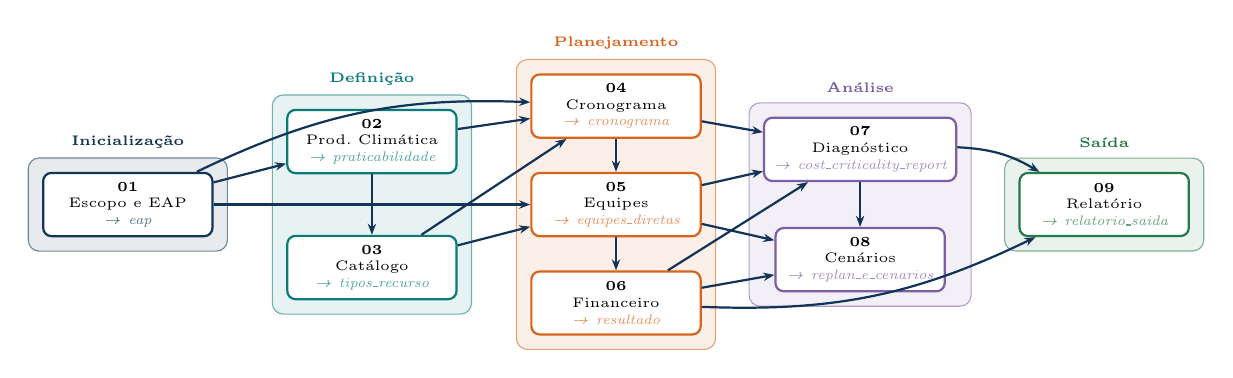
\begin{tikzpicture}[
      skill/.style={draw,fill=white,rounded corners=3pt,
                    minimum width=2.15cm,minimum height=0.8cm,align=center,
                    font=\tiny,line width=0.8pt},
      arr2/.style={-{Stealth[length=4pt]},mlblue,thick},
      ph/.style={rounded corners=4pt,inner sep=5pt},
      phlbl/.style={font=\tiny\bfseries,anchor=south},
    ]
    % ── nós (uma coluna por fase) ─────────────────────────────────────────
    % Tag "→ artefato" = [produces].canonical_section do skill.toml --- o
    % que o nó exporta para TODOS os sucessores (espinha e depends_on).
    \node[skill,draw=mlblue]   (s1) at (0,0)
      {\textbf{01}\\Escopo e EAP\\{\tiny\textit{\textcolor{mlblue!70}{→ eap}}}};
    \node[skill,draw=mlteal]   (s2) at (3.1,0.8)
      {\textbf{02}\\Prod.\ Climática\\{\tiny\textit{\textcolor{mlteal!70}{→ praticabilidade}}}};
    \node[skill,draw=mlteal]   (s3) at (3.1,-0.8)
      {\textbf{03}\\Catálogo\\{\tiny\textit{\textcolor{mlteal!70}{→ tipos\_recurso}}}};
    \node[skill,draw=mlorange] (s4) at (6.2,1.25)
      {\textbf{04}\\Cronograma\\{\tiny\textit{\textcolor{mlorange!70}{→ cronograma}}}};
    \node[skill,draw=mlorange] (s5) at (6.2,0)
      {\textbf{05}\\Equipes\\{\tiny\textit{\textcolor{mlorange!70}{→ equipes\_diretas}}}};
    \node[skill,draw=mlorange] (s6) at (6.2,-1.25)
      {\textbf{06}\\Financeiro\\{\tiny\textit{\textcolor{mlorange!70}{→ resultado}}}};
    \node[skill,draw=mlpurple] (s7) at (9.3,0.7)
      {\textbf{07}\\Diagnóstico\\{\fontsize{4}{4.5}\selectfont\textit{\textcolor{mlpurple!70}{→ cost\_criticality\_report}}}};
    \node[skill,draw=mlpurple] (s8) at (9.3,-0.7)
      {\textbf{08}\\Cenários\\{\fontsize{4}{4.5}\selectfont\textit{\textcolor{mlpurple!70}{→ replan\_e\_cenarios}}}};
    \node[skill,draw=mlgreen]  (s9) at (12.4,0)
      {\textbf{09}\\Relatório\\{\tiny\textit{\textcolor{mlgreen!70}{→ relatorio\_saida}}}};
    % ── clusters de fase (atrás dos nós) ──────────────────────────────────
    \begin{scope}[on background layer]
      \node[ph,fill=mlblue!10,draw=mlblue!60,fit=(s1)]      (ph1) {};
      \node[ph,fill=mlteal!10,draw=mlteal!60,fit=(s2)(s3)]  (ph2) {};
      \node[ph,fill=mlorange!10,draw=mlorange!60,fit=(s4)(s5)(s6)] (ph3) {};
      \node[ph,fill=mlpurple!10,draw=mlpurple!60,fit=(s7)(s8)]     (ph4) {};
      \node[ph,fill=mlgreen!10,draw=mlgreen!60,fit=(s9)]    (ph5) {};
    \end{scope}
    \node[phlbl,mlblue]   at (ph1.north) {Inicialização};
    \node[phlbl,mlteal]   at (ph2.north) {Definição};
    \node[phlbl,mlorange] at (ph3.north) {Planejamento};
    \node[phlbl,mlpurple] at (ph4.north) {Análise};
    \node[phlbl,mlgreen]  at (ph5.north) {Saída};
    % ── todas as arestas: depends_on real declarado no skill.toml ─────────
    \draw[arr2] (s1) -- (s2);
    \draw[arr2] (s2) -- (s3);
    \draw[arr2] (s3) -- (s4);
    \draw[arr2] (s4) -- (s5);
    \draw[arr2] (s5) -- (s6);
    \draw[arr2] (s6) -- (s7);
    \draw[arr2] (s7) -- (s8);
    \draw[arr2] (s1) to[bend left=14] (s4);
    \draw[arr2] (s2) -- (s4);
    \draw[arr2] (s1) -- (s5);
    \draw[arr2] (s3) -- (s5);
    \draw[arr2] (s4) -- (s7);
    \draw[arr2] (s5) -- (s7);
    \draw[arr2] (s5) -- (s8);
    \draw[arr2] (s6) -- (s8);
    \draw[arr2] (s7) to[bend left=14] (s9);
    \draw[arr2] (s6) to[bend right=14] (s9);
  \end{tikzpicture}}
  \vspace{2pt}
  \raggedright
  \begin{columns}[T]
    \column{0.5\textwidth}
    \begin{itemize}\tiny
      \item 9 skills, todas ativas, 01--09 contíguo na ordem de execução
      \item Setas: \texttt{depends\_on} real de cada skill --- 09 lê
            06/07, não depende de 08
      \item \texttt{→ artefato} sob cada nó: seção canônica exportada
            (\texttt{[produces]}), consumida por todo sucessor
    \end{itemize}
    \column{0.5\textwidth}
    \begin{itemize}\tiny
      \item Estrutura 1:1 com \texttt{concilium configuration skills
            export -{}-group-by-phase}
      \item Tudo é congelado e versionado a cada execução
    \end{itemize}
  \end{columns}
\end{frame}

\subsection{Catálogo}

\lvlA
\begin{frame}
  \mtitle{Catálogo: Modelagem de Dados}
  \centering
  % ── Banda 1: ContextoObra resolve a configuração da obra ──────────────────
  \resizebox{0.82\linewidth}{!}{%
  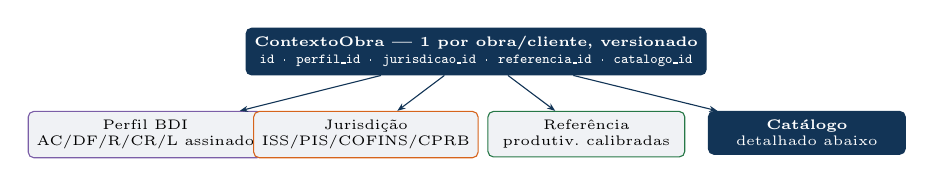
\begin{tikzpicture}[
      box/.style={draw=mlblue,fill=mlgray,rounded corners=2pt,font=\tiny,
                  align=center,inner sep=3pt,minimum width=2.5cm},
      arr2/.style={-{Stealth[length=3pt]},mlblue},
    ]
    \node[box,fill=mlblue,text=white,minimum width=5.6cm] (ctx)
      {\textbf{ContextoObra --- 1 por obra/cliente, versionado}\\
       \texttt{id · perfil\_id · jurisdicao\_id · referencia\_id · catalogo\_id}};
    \node[box,below=0.45cm of ctx,xshift=-4.2cm,draw=mlpurple] (bdi) {Perfil BDI\\AC/DF/R/CR/L assinado};
    \node[box,below=0.45cm of ctx,xshift=-1.4cm,draw=mlorange] (jur) {Jurisdição\\ISS/PIS/COFINS/CPRB};
    \node[box,below=0.45cm of ctx,xshift=1.4cm,draw=mlgreen]  (ref) {Referência\\produtiv.\ calibradas};
    \node[box,below=0.45cm of ctx,xshift=4.2cm,fill=mlblue,text=white] (cat) {\textbf{Catálogo}\\detalhado abaixo};
    \foreach \n in {bdi,jur,ref,cat} \draw[arr2] (ctx) -- (\n);
  \end{tikzpicture}}\\[4pt]
  % ── Banda 2: espinha real de catálogo CPU → Producao → Insumo → {MO,EQ,MAT}
  % (4 níveis, lidos de cima para baixo). CPU/Producao/Insumo são as 3
  % entidades/pastas reais de catálogo (cpus, produtividades, insumos);
  % MO/EQ/MAT fecham a cadeia como composicao_padrao_equipe, estrutura
  % interna de Producao que referencia Insumo (fan-in).
  %
  % Atualizado 2026-07-21: MO/EQ/MAT são ids soltos (sem FK de banco) --- a
  % integridade é 100% de aplicação. As 3 referências (funcao_id/equip_id/
  % insumo_id) hoje derivam de um registro único (catalog_refs.py) e são
  % checadas por VAL-CPU-INS-06/07/08 dentro do gate obrigatório ADR-035
  % (assert_catalog_healthy, bloqueia avancar_plano). Antes desta data,
  % materiais.insumo_id (MAT) não tinha checagem nenhuma nos dois
  % validadores existentes --- o mesmo buraco em ambos, por falta de fonte
  % única. Removida também a menção a uma entidade "Funcao" intermediária
  % entre funcao_id e Insumo: esse modelo existe em código (catalogo.py)
  % mas é órfão --- nenhum repositório/config o usa; funcao_existe() resolve
  % funcao_id direto contra Insumo(tipo=MAO_OBRA), sem esse hop.
  %
  % Adicionada seta Producao -> Insumo direta para materiais_gerados[]
  % (ADR-139, lado produtor: MaterialGerado.insumo_id, VAL-PROD-GERACAO-01).
  % Essa é a ÚNICA referência direta de Producao a Insumo --- diferente de
  % MO/EQ/MAT, que são fan-in via itens embutidos, não uma referência única.
  % O campo já aparecia no texto do node Producao mas faltava a seta.
  %
  % Removida a seta curva "contém (embutido, sem FK de banco)" de Producao
  % até a zona MO/EQ/MAT: decisão de simplificação de apresentação (não de
  % precisão) --- o fato de containment já está dito em texto no label da
  % zona2 ("dentro de Producao") e reforçado pelas 3 setas FK app convergindo
  % em Insumo. Era a linha mais complexa do diagrama (contornava Insumo) só
  % para repetir algo já expresso em palavras.
  %
  % Bloco "Como o PU nasce" simplificado para citar só Fonte 1 (bottom-up via
  % equipe de Producao) --- decisão de apresentação, Fonte 2 (fallback via
  % composicao_itens, só quando F1 falha) continua real no código
  % (_resolve_preco_cat_item, NEP-032 D1) e ainda aparece no diagrama via a
  % seta "FK: composicao_itens.insumo_id (fallback)" perto de CPU.
  \begin{columns}[T]
    \column{0.48\textwidth}
    \resizebox{!}{4.3cm}{%
    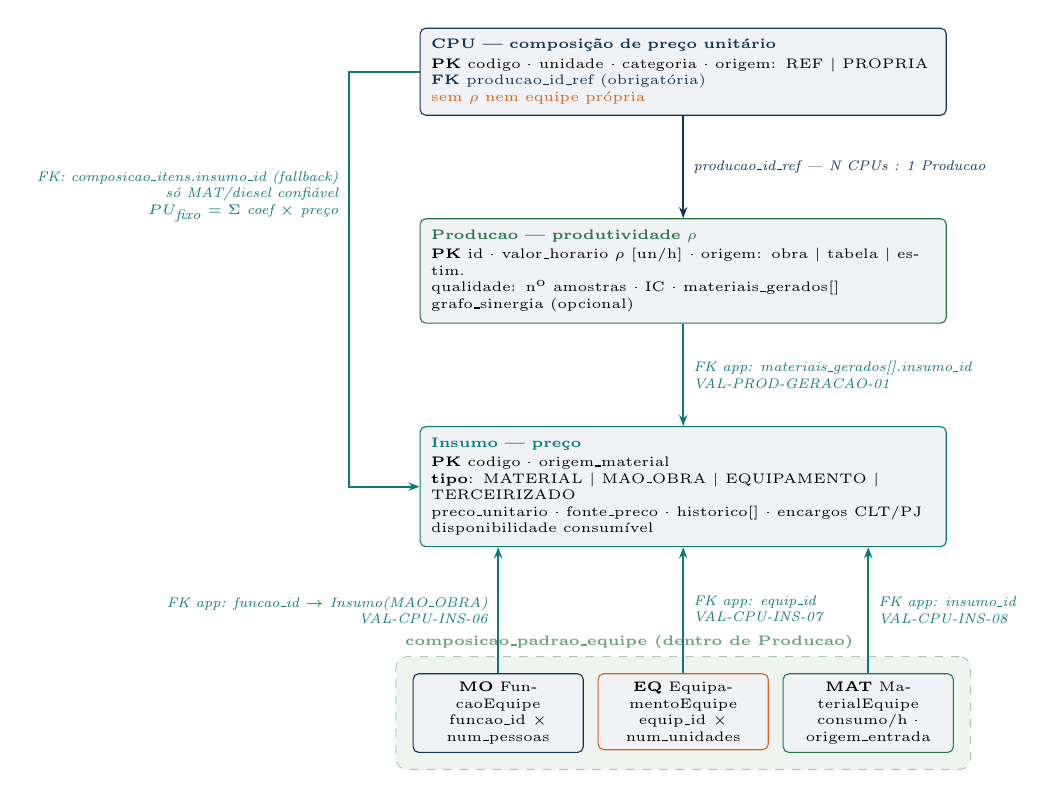
\begin{tikzpicture}[
        ent/.style={draw,fill=mlgray,rounded corners=2pt,font=\tiny,
                    align=left,inner sep=4pt,text width=6.4cm},
        chip/.style={draw,fill=mlgray,rounded corners=2pt,font=\tiny,
                     align=center,inner sep=3pt,text width=1.95cm},
        rel/.style={-{Stealth[length=4pt]},thick},
        lbl/.style={font=\tiny\itshape},
        zona2/.style={rounded corners=4pt,inner sep=6pt},
      ]
      \node[ent,draw=mlblue] (cpu)
        {\textbf{\textcolor{mlblue}{CPU --- composição de preço unitário}}\\[1pt]
         \textbf{PK} codigo · unidade · categoria · origem: REF $|$ PROPRIA\\
         \textcolor{mlblue}{\textbf{FK} producao\_id\_ref (obrigatória)}\\
         \textcolor{mlorange}{sem $\rho$ nem equipe própria}};
      \node[ent,draw=mlgreen,below=1.3cm of cpu] (pro)
        {\textbf{\textcolor{mlgreen}{Producao --- produtividade $\rho$}}\\[1pt]
         \textbf{PK} id · valor\_horario $\rho$ [un/h] · origem: obra $|$ tabela $|$ estim.\\
         qualidade: n\textsuperscript{o} amostras · IC · materiais\_gerados{[]}\\
         grafo\_sinergia (opcional)};
      \node[ent,draw=mlteal,below=1.3cm of pro] (ins)
        {\textbf{\textcolor{mlteal}{Insumo --- preço}}\\[1pt]
         \textbf{PK} codigo · origem\_material\\
         \textbf{tipo}: MATERIAL $|$ MAO\_OBRA $|$ EQUIPAMENTO $|$ \mbox{TERCEIRIZADO}\\
         preco\_unitario · fonte\_preco · historico{[]} · encargos CLT/PJ\\
         disponibilidade consumível};
      % ── MO/EQ/MAT: última camada da cadeia, estrutura interna de Producao ─
      \node[chip,draw=mlblue,below=1.6cm of ins,xshift=-2.35cm] (mo)
        {\textbf{MO} FuncaoEquipe\\funcao\_id $\times$ num\_pessoas};
      \node[chip,draw=mlorange,below=1.6cm of ins] (eq)
        {\textbf{EQ} EquipamentoEquipe\\equip\_id $\times$ num\_unidades};
      \node[chip,draw=mlgreen,below=1.6cm of ins,xshift=2.35cm] (mat)
        {\textbf{MAT} MaterialEquipe\\consumo/h · origem\_entrada};
      \begin{scope}[on background layer]
        \node[zona2,fill=mlgreen!8,draw=mlgreen!40,dashed,fit=(mo)(eq)(mat),
              label={[font=\tiny\bfseries,text=mlgreen!70,anchor=south west,
              yshift=-1pt]north west:composicao\_padrao\_equipe (dentro de Producao)}]
              (zona2) {};
      \end{scope}
      % ── espinha vertical: CPU → Producao → Insumo → {MO,EQ,MAT} ──────────
      \draw[rel,mlblue] (cpu) -- node[lbl,right]{producao\_id\_ref --- N CPUs : 1 Producao} (pro);
      \draw[rel,mlteal] (pro.south) -- node[lbl,right,align=left]{FK app: materiais\_gerados[].insumo\_id\\VAL-PROD-GERACAO-01} (ins.north);
      \draw[rel,mlteal] (mo.north) -- node[lbl,left,align=right]{FK app: funcao\_id \arr\ Insumo(MAO\_OBRA)\\VAL-CPU-INS-06} (mo.north |- ins.south);
      \draw[rel,mlteal] (eq.north) -- node[lbl,right,align=left]{FK app: equip\_id\\VAL-CPU-INS-07} (ins.south);
      \draw[rel,mlteal] (mat.north) -- node[lbl,right,align=left]{FK app: insumo\_id\\VAL-CPU-INS-08} (mat.north |- ins.south);
      \draw[rel,mlteal] (cpu.west) -- ++(-0.9,0) |-
        node[lbl,left,pos=0.15,align=right]
        {FK: composicao\_itens.insumo\_id (fallback)\\só MAT/diesel confiável\\$PU_{\text{fixo}} = \Sigma$ coef $\times$ preço}
        (ins.west);
    \end{tikzpicture}}
    \column{0.48\textwidth}
    \begin{block}{\small Como o PU nasce}
      \scriptsize
      \centerline{$p_i^c = \frac{\gamma_i}{\rho_i}$}
      \smallskip

      $\gamma_i$: custo horário da equipe (MO + EQ + diesel + MAT), bottom-up
      via composição de Producao\\
      $\rho_i$: valor horário da produção
    \end{block}
    \vspace{1pt}
    \begin{block}{\small Integridade e resolução de preço}
      \scriptsize
      \textbf{funcao\_id / equip\_id / insumo\_id} --- sem FK de banco;
      checados por VAL-CPU-INS-06/07/08\\[2pt]
      \textbf{N CPUs : 1 Producao} --- nunca duplica \\[2pt]
      \textbf{Snapshot}: sem cópia integral --- guarda
      \texttt{catalogo\_id}; CPUs resolvidas sob demanda
    \end{block}
  \end{columns}
\end{frame}

\lvlA
\begin{frame}
  \mtitle{Equipe-Padrão: Composição}
  \begin{columns}[T]
    \column{0.55\textwidth}
    \begin{block}{Três tipos de recurso ($e_i$)}
      \scriptsize
      \begin{tabular}{@{}lll@{}}
        \textbf{MO}  & Operador de máquina & $\times 1$ \\
                     & Auxiliar de operação & $\times 2$ \\
        \textbf{EQ}  & Retroescavadeira & $\times 1$ \\
                     & Caminhão basculante & $\times 1$ \\
        \textbf{MAT} & Geotêxtil Bidim OP-30 & 327,5 m\textsuperscript{2}/h \\
      \end{tabular}
    \end{block}
    \vspace{4pt}
    \begin{block}{Custo horário}
      \vspace{-4pt}
      \[
        \gamma_i = \sum_{r \in R_i} n_r \cdot \gamma_r
        \;+\; \underbrace{\sum_{e \in R_i^{EQ}} n_e \cdot f_e \cdot c_{\text{dsl}}}_{\gamma_i^{\text{comb}}}
      \]
      \vspace{-6pt}
      \begin{itemize}\scriptsize\setlength{\itemsep}{0pt}\setlength{\topsep}{0pt}\setlength{\parskip}{0pt}
        \item $n_r$: qtd/equipe
        \item $\gamma_r$: custo/hora de $r$
        \item $f_e$: consumo de combustível [un${}^{\text{comb}}$/h]
        \item $c_{e}^{\text{comb}}$: preço do litro --- API ANP por UF; offline \arr\ R\$~6,50/l
      \end{itemize}
    \end{block}
    \column{0.4\textwidth}
    \begin{block}{Composição formal}
      \[
        e_i = (R_i^{MO}, R_i^{EQ}, R_i^{MAT})
      \]
      \[
        R_i^{*} = \{(r, n_r)\}_r
      \]
    \end{block}
    \vspace{4pt}
    \begin{block}{Slots no pool}
      \[
        |\mathcal{E}_i^r| = m_i^{*} \cdot n_r
      \]
      $m_i^{*}$: pico de equipes simultâneas
    \end{block}
  \end{columns}
\end{frame}

\begin{frame}
  \mtitle{Equipe-Padrão: Grafo de Sinergia e Produtividade Derivada}
  \begin{columns}[T]
    \column{0.55\textwidth}
    \begin{block}{Capacidade efetiva e gargalo}
      \[
        \rho^{\text{sin}} = \min_e\,(k_e \cdot n_e)
      \]
      \scriptsize $k_e n_e$: capacidade efetiva do elemento $e$.\\
      Gargalo = argmin --- não é soma, é o elo mais fraco.
    \end{block}
    \vspace{4pt}
    \begin{block}{Tipos de relação}
      \scriptsize
      \textbf{acoplamento}: grupo opera no mín.\ dos $k_e n_e$\\
      \textbf{dimensionamento}: destino satura no $k_e n_e$ da origem\\
      \textbf{precondição}: só habilita, não define taxa
    \end{block}
    \column{0.4\textwidth}
    \begin{block}{Exemplo real (catálogo)}
      \resizebox{\linewidth}{!}{%
      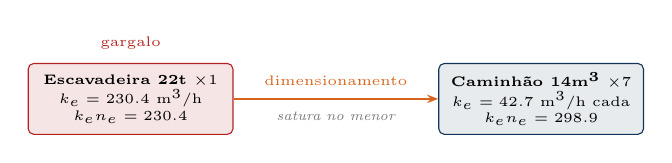
\begin{tikzpicture}[
          box/.style={draw,fill=mlgray,rounded corners=2pt,font=\tiny,
                      align=center,inner sep=3pt,minimum width=2.6cm,minimum height=0.9cm},
          arr2/.style={-{Stealth[length=4pt]},mlorange,thick},
        ]
        \node[box,draw=mlred,fill=mlred!12] (esc) {\textbf{Escavadeira 22t} $\times$1\\$k_e = 230.4$ m\textsuperscript{3}/h\\$k_e n_e = 230.4$};
        \node[box,right=2.6cm of esc,draw=mlblue,fill=mlblue!10] (cam) {\textbf{Caminhão 14m\textsuperscript{3}} $\times$7\\$k_e = 42.7$ m\textsuperscript{3}/h cada\\$k_e n_e = 298.9$};
        \draw[arr2] (esc) -- node[above=1pt,font=\tiny,mlorange]{dimensionamento}
                             node[below=1pt,font=\tiny\itshape,mlgray!50!black]{satura no menor} (cam);
        \node[font=\tiny,mlred,above=0.05cm of esc] {gargalo};
      \end{tikzpicture}}\\[4pt]
      {\scriptsize $\rho^{\text{sin}} = \min(230.4,\, 298.9) = 230.4$
      m\textsuperscript{3}/h --- bate com o declarado (231.87, $<$1\%).}
    \end{block}
  \end{columns}
\end{frame}

\lvlA
\begin{frame}
  \mtitle{Processo de Atualização de Catálogo: Regra dos Quatro Olhos}
  \begin{columns}[T]
    \column{0.5\textwidth}
    \begin{block}{Fontes}
      \begin{itemize}\scriptsize
        \item SINAPI
        \item Pesquisa de mercado
        \item Calibração por obra
        \item Mudança tributária
      \end{itemize}
    \end{block}
    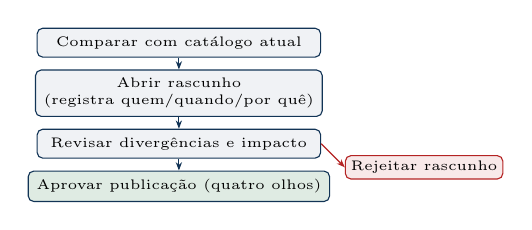
\begin{tikzpicture}[
        box/.style={draw=mlblue,fill=mlgray,rounded corners=2pt,
                    minimum width=3.6cm,font=\tiny,align=center,
                    inner sep=3pt},
        boxr/.style={draw=mlred,fill=mlred!10,rounded corners=2pt,
                     minimum width=1.9cm,font=\tiny,align=center,
                     inner sep=2pt},
        arr2/.style={-{Stealth[length=3pt]},mlblue},
      ]
      \node[box] (c1) {Comparar com catálogo atual};
      \node[box,below=0.15cm of c1] (c2) {Abrir rascunho\\(registra quem/quando/por quê)};
      \node[box,below=0.15cm of c2] (c3) {Revisar divergências e impacto};
      \node[box,below=0.15cm of c3,fill=mlgreen!15] (c4) {Aprovar publicação (quatro olhos)};
      \node[boxr,right=0.3cm of c3,yshift=-0.3cm] (c3b) {Rejeitar rascunho};
      \draw[arr2] (c1) -- (c2);
      \draw[arr2] (c2) -- (c3);
      \draw[arr2] (c3) -- (c4);
      \draw[arr2,mlred] (c3.east) -- (c3b.west);
    \end{tikzpicture}
    \begin{minipage}{0.9\linewidth}
      \raggedright\tiny\itshape Aprovar exige
      revisão prévia; rejeitado, já aprovado, ou mesmo ator
      criando/aprovando são bloqueados.
    \end{minipage}
    \column{0.44\textwidth}
    \begin{alertblock}{\small Regra dos quatro olhos}
      \scriptsize Quem cria \textbf{não} pode aprovar o próprio rascunho ---
      checado por ator (\texttt{created\_by} vs.\ aprovador), não só por
      role.\\
      Rascunho rejeitado fica bloqueado (não pode ser reaprovado).
    \end{alertblock}
    \vspace{4pt}
    \begin{exampleblock}{\small Isolamento de projetos}
      \scriptsize Nova versão do catálogo \textbf{não} afeta projetos
      existentes --- cada projeto guarda a versão que usou. Aplicar
      preços novos é uma decisão explícita: cria-se novo plano e
      compara-se o resultado.
    \end{exampleblock}
  \end{columns}
\end{frame}

\subsection{Cronograma: Precedências e quantitativos}
\begin{frame}
  \mtitle{Modelagem do Cronograma: Duração e Precedências}
  \begin{columns}[T]
    \column{0.5\textwidth}
    \begin{exampleblock}{\small Cronograma: Otimização}
      \scriptsize
      \[
        \min\,\text{prazo} \;\;\text{s.a.}\;\; \theta,\, S_r(t),\, \lambda_j
      \]
      \emph{Resource-Constrained Project Scheduling Problem (RCPSP)} --- NP-hard
    \end{exampleblock}
    \vspace{4pt}
    \begin{block}{Precedência: limiar de completude}
      \[
        \text{start}_j \geq \text{start}_i + \lceil \theta_i \cdot \Delta t_i \rceil
      \]
      \scriptsize $\theta_i \in [0,1]$: fração da duração de $i$ (não do
      acumulado \% de equipes). $\theta=1$: precedência completa.
    \end{block}
    \column{0.44\textwidth}
    \begin{block}{Envelope e duração produtiva}
      \[
        \Delta t_i = \left\lceil \frac{Q_i}{\rho_i} \right\rceil
      \]
    \end{block}
    \vspace{4pt}
    \begin{block}{Ramp semanal e mob/demob}
      \[
        m_{ij} = \text{round}(m_i^{\text{pico}} \cdot \text{ramp}_{ij})
      \]
      \[
        q_{ij} = m_{ij} \cdot \rho_i \cdot \lambda_j \cdot d_j \cdot h_j
      \]
      \begin{itemize}\scriptsize
        \item $\lambda_j$: eficiência de clima
        \item $d_j$: dias produtivos da semana
        \item rampa já embutida em $m_{ij}$
        \item {[M]/[D]}: início/fim de cadeia de slots
      \end{itemize}
    \end{block}
  \end{columns}
\end{frame}

\subsection{Banco de recursos}

\lvlA
\begin{frame}
  \mtitle{Pool de Recursos: Reaproveitamento de Equipes}
  \begin{columns}[T]
    \column{0.55\textwidth}
    \resizebox{\linewidth}{!}{%
    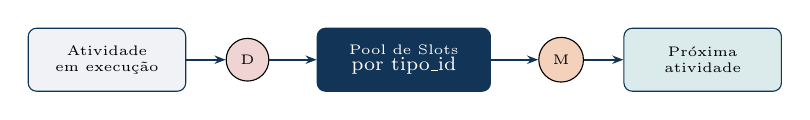
\begin{tikzpicture}[
        box/.style={draw=mlblue,fill=mlgray,rounded corners=3pt,font=\tiny,
                    align=center,inner sep=3pt,minimum height=0.8cm},
        arr2/.style={-{Stealth[length=4pt]},mlblue,thick},
      ]
      \node[box,minimum width=2.0cm] (a1) {Atividade\\em execução};
      \node[draw,circle,fill=mlred!20,right=0.5cm of a1,font=\tiny] (d) {D};
      \node[box,fill=mlblue,text=white,right=0.6cm of d,minimum width=2.2cm] (pool) {Pool de Slots\\\scriptsize por tipo\_id};
      \node[draw,circle,fill=mlorange!30,right=0.6cm of pool,font=\tiny] (m) {M};
      \node[box,minimum width=2.0cm,right=0.5cm of m,fill=mlteal!15] (a2) {Próxima\\atividade};
      \draw[arr2] (a1) -- (d);
      \draw[arr2] (d) -- (pool);
      \draw[arr2] (pool) -- (m);
      \draw[arr2] (m) -- (a2);
    \end{tikzpicture}}\\[6pt]
    {\scriptsize\itshape Pool perpétuo --- persiste entre atividades da
    cadeia, no escopo do projeto. Slots só entram via desmobilização.}
      \column{0.4\textwidth}
    \begin{alertblock}{Sem pool}
      \begin{itemize}\scriptsize
        \item 1 mob+demob por atividade
        \item $c_{\text{mob}}>0$ sempre
        \item perda de aprendizado
      \end{itemize}
    \end{alertblock}
    \vspace{4pt}
    \begin{exampleblock}{Com pool}
      \begin{itemize}\scriptsize
        \item 1 mob+demob por \textbf{cadeia}
        \item $c_{\text{mob}}=0$ ao reaproveitar
        \item know-how preservado
      \end{itemize}
    \end{exampleblock}
  \end{columns}
\end{frame}

\lvlA
\begin{frame}
  \mtitle{Pool: Ciclo de Vida dos Slots ao Longo das Atividades}
  \begin{columns}[T]
    \column{0.55\textwidth}
    \begin{block}{Cadeia 1 --- tipo ESC (exemplo)}
      \scriptsize Pavim.\ A (S1--4) \arr\ \textit{standby}
      \arr\ Pavim.\ B (S6--8) \arr\ \textit{standby} \arr\
      Pavim.\ C (S10--12)\\[4pt]
      \textbf{1 mob total $\cdot$ 1 demob total $\cdot$ $c_{\text{mob}}$ cobrado 1$\times$}
    \end{block}
    \vspace{4pt}
    \begin{block}{Standby}
      \scriptsize Slot permanece \texttt{NO POOL} entre atividades da
      mesma cadeia, sempre dentro do mesmo projeto (pool isolado por
      \texttt{projeto\_id}); custo $\kappa \cdot c_{\text{eq}}$/semana
      (equipamento parado, não desmobilizado).
    \end{block}
    \column{0.4\textwidth}
    \begin{alertblock}{Sem pool}
      \begin{itemize}\scriptsize
        \item $n_{\text{ativ}}\times$ mob/demob
        \item sem standby
        \item perda de aprendizado
      \end{itemize}
    \end{alertblock}
    \vspace{4pt}
    \begin{exampleblock}{Com pool}
      \begin{itemize}\scriptsize
        \item 1$\times$ mob/demob por cadeia
        \item $\kappa c_{\text{eq}} n_{\text{standby}}$
        \item MO retido/dispensado
      \end{itemize}
    \end{exampleblock}
  \end{columns}
\end{frame}

\lvlA
\begin{frame}
  \mtitle{Banco de Recursos: Consumíveis e Repropagação de Atraso}
  \begin{columns}[T]
    \column{0.5\textwidth}
    \begin{block}{Recurso do pool \emph{vs.}\ recurso consumível}
      \begin{columns}[T]
        \column{0.48\linewidth}
        {\scriptsize\textbf{\textcolor{mlblue}{Recurso do pool}}}
        \begin{itemize}\scriptsize
          \item contagem de unidades
          \item mob $\to$ uso $\to$ demob $\to$ volta
          \item nunca se esgota
          \item ex.: escavadeira, operador
        \end{itemize}
        \column{0.48\linewidth}
        {\scriptsize\textbf{\textcolor{mlorange}{Recurso consumível}}}
        \begin{itemize}\scriptsize
          \item fluxo/estoque
          \item consumido, não retorna
          \item precisa reabastecer
          \item ex.: diesel, material
        \end{itemize}
      \end{columns}
    \end{block}
    \vspace{6pt}
    \begin{block}{Disponibilidade consumível}
      \begin{itemize}\scriptsize
        \item $K$: capacidade de armazenamento (tanque/pilha)
        \item $E_0$: estoque inicial
        \item $a_{\max}$: taxa máx.\ de abastecimento externo
        \item lead time de reabastecimento [dias]
      \end{itemize}
    \end{block}
    \column{0.44\textwidth}
    \begin{block}{Projeção semanal de estoque}
      \[
        E_t = \min(E_{t-1} + a_{\max} + g_t,\, K) - u_t
      \]
      \scriptsize $E_t<0$ em alguma semana $\to$ cronograma inviável como está\\
      \scriptsize $a_{\max}$: abastecimento externo $\cdot$ $g_t$: produção
      \emph{interna} das frentes ativas --- o produtor-consumidor;
      $u_t$: consumo; excedente sobre $K$ é descartado (aviso, não delay).
    \end{block}
    \vspace{4pt}
    \begin{exampleblock}{\small Reparo por atraso}
      \scriptsize
      1. Atrasa a atividade consumidora até $E_t \geq 0$.\\
      2. Repropaga precedências: empurra sucessores no DAG
      (nunca antecipa).\\
      Os dois passos alternam até ponto fixo (máx.\ 10 rounds).\\
      \textbf{Contabilização} (resumo por recurso $+$ cubo semanal $+$
      MCP/REST) em paridade com pool.
    \end{exampleblock}
  \end{columns}
\end{frame}

\lvlA
\begin{frame}
  \mtitle{Materiais Consumíveis: Origem e Produtor--Consumidor}
  \begin{columns}[T]
    \column{0.5\textwidth}
    \begin{block}{Origem — ortogonal ao tipo}
      \scriptsize
      Todo material é de \textbf{aquisição externa} ou de
      \textbf{geração interna}:\\[2pt]
      compra (areia, CAP, tubos) $\times$ gerado pela obra (solo de
      corte, massa usinada). Cotação/tendência de preço só para compra.
    \end{block}
    \vspace{4pt}
    \begin{block}{Lado produtor no catálogo}
      \scriptsize A frente declara no catálogo o que \textbf{gera} por
      hora, simétrico ao que consome ($g$ $\times$ $u$); a física fica
      no catálogo, o pareamento frente\,\arr\,estoque é dado de projeto.
    \end{block}
    \column{0.44\textwidth}
    \begin{block}{Efeito real}
      \scriptsize BGTC: 92{,}50 \arr\ \textbf{245{,}63 R\$/m³}\\
      CBUQ: 385 \arr\ \textbf{466{,}30 R\$/t}\\
      \tiny cotações da empresa; referência SICRO 202604 registrada na
      conclusão de preço; recotação re-conclui.
    \end{block}
    \vspace{4pt}
    \begin{block}{Scheduler}
      \scriptsize consumidora mais rápida que a produtora \arr\ delay
      até o estoque acumular; a produtora nunca é atrasada.
    \end{block}
  \end{columns}
\end{frame}

\subsection{Regras de negócio}

\lvlA
\begin{frame}
  \mtitle{Custo Operacional e de Banco de Recursos}
  \begin{columns}[T]
    \column{0.48\textwidth}
    \begin{block}{Custo horário e eficiência de planejamento}
      \footnotesize
      $\displaystyle\gamma_i = \sum_{r \in R_i} n_r \gamma_r
      \quad \eta_j = \lambda_j \cdot \delta_j$
      \vspace{1pt}

      \scriptsize Decomposto: MO, EQ, combustível, material.
      Eficiência: $\lambda_j$ clima $\times$ $\delta_j$ dias produtivos.
    \end{block}
    \vspace{2pt}
    \begin{block}{Custo por ciclo de vida da equipe}
      \scriptsize
      \vspace{-6pt}
      \begin{align*}
        C_{\text{prod},i} &= \gamma_i\, n_p\\
        C_{\text{pool},i} &= C_{\text{prod},i} + (\gamma_i^{mo} + \kappa\gamma_i^{eq})\, n_s\\
        \tilde{C}_i       &= C_{\text{pool},i} + c_{\text{mob}} + c_{\text{dem}}
      \end{align*}
      \vspace{-14pt}

      \tiny $n_p$: sem.\ produtivas $\cdot$ $n_s$: sem.\ standby $\cdot$ MO
      integral $\cdot$ EQ $\kappa\gamma_i^{eq}$, $\kappa\leq1$\\
      \textbf{\scriptsize $C_{\text{prod}} \leq C_{\text{pool}} \leq$ custo total}
    \end{block}
    \column{0.46\textwidth}
    \begin{columns}[T]
      \column{0.48\textwidth}
      \begin{block}{\scriptsize Catálogo}
        \[
          p_i^c = \frac{\gamma_i}{\rho_i}
        \]
      \end{block}
      \column{0.48\textwidth}
      \begin{block}{\scriptsize Operacional}
        \[
          p_i^o = \frac{C_{\text{pool},i}}{Q_i}
        \]
      \end{block}
    \end{columns}
    \vspace{4pt}
    \begin{block}{Relação catálogo $\times$ operacional}
      \[
        p_i^o = p_i^c \cdot \tau_i
      \]
      \scriptsize dois efeitos opostos: perda de eficiência
      (clima/calendário) empurra $\tau_i$ acima de 1; partilha de pool e
      reaproveitamento empurram abaixo (
      $C_{\text{inst}} \leq$ catálogo).
    \end{block}
  \end{columns}
\end{frame}

\lvlA
\lvlB
\begin{frame}
  \mtitle{BDI: Composição e Valor de Venda}
  \begin{columns}[T]
    \column{0.48\textwidth}
    \begin{block}{Fórmula do BDI (base TCU, Acórdão 2622/2013)}
      \resizebox{0.98\linewidth}{!}{$
        \beta = \dfrac{(1+AC)(1+DF)(1+R)(1+CR)(1+L)}{1-T} - 1
      $}
      \scriptsize AC adm.\ central $\cdot$ DF desp.\ financeiras $\cdot$ R
      risco/seguro/garantia $\cdot$ CR contingência $\cdot$ L lucro $\cdot$
      T tributos (PIS+COFINS+ISS+CSLL+IR). Composição multiplicativa,
      \textbf{BDI por categoria de custo}.
    \end{block}
    \vspace{2pt}
    \begin{block}{Valor de venda}
      \scriptsize
      Direto: $V_i^D = \sum_{j}\sum_{r \in A_i} \beta_r \gamma_r h\, d\, m_{ij}$\\[2pt]
      Indireto:
      $V_i^I = \sum_{j}\sum_{q \in B_i} \beta_q \gamma_q h\, d$
    \end{block}
    \column{0.46\textwidth}
    \begin{exampleblock}{\small Memorial de cálculo}
      \scriptsize Trilha auditável: salário $\to$ encargos $\to$ custo
      $\to$ BDI $\to$ preço de venda. Assinatura de integridade
      (hash) por versão do perfil.
    \end{exampleblock}
    \vspace{4pt}
    \begin{block}{Três níveis de custo}
      \begin{enumerate}\scriptsize
        \item Equipes isoladas
        \item Com pool partilhado
        \item Custo final por ciclo de vida --- cada nível rastreável
      \end{enumerate}
    \end{block}
  \end{columns}
\end{frame}

\lvlB
\begin{frame}
  \mtitle{BDI: Composição de Tributos por Jurisdição e Categoria}
  \begin{columns}[T]
    \column{0.48\textwidth}
    \begin{block}{Motor tributário por jurisdição}
      \scriptsize Antes: alíquota média/flat --- risco fiscal em
      praças de ISS alto. Agora: \texttt{Escopo.jurisdicao\_id}
      resolve as alíquotas reais do local.\\[4pt]
      \texttt{AliquotasBdi} = \{ISS, PIS, COFINS, CPRB\} por
      \texttt{config/jurisdicoes/BR-\{UF\}}
    \end{block}
    \vspace{4pt}
    \begin{block}{Exemplo: duas UFs, mesma obra}
      \scriptsize
      \begin{tabular}{@{}lcc@{}}
        & BR-CE & BR-SP \\
        ISS     & 2\%    & 5\% (LC 116/2003, teto) \\
        PIS     & 0.65\% & 0.65\% \\
        COFINS  & 3\%    & 3\% \\
        CPRB    & 4.5\%  & 4.5\% (desoneração setorial) \\
      \end{tabular}\\[4pt]
      Só o ISS muda entre as praças (resolvido por UF no modelo) --- mas
      isso já move o BDI final.
    \end{block}
    \column{0.46\textwidth}
    \begin{exampleblock}{\small Tributo varia por categoria --- por que importa}
      \begin{itemize}\scriptsize
        \item \textcolor{mlorange}{Serviço} (MO, aluguel, manutenção):
          BDI $\approx$29.97\% (ISS 5\%+CSLL+IR+AC/DF/R+L)
        \item \textcolor{mlgreen}{Material/diesel} (mercadoria): BDI
          = 4\% (só lucro --- sem ISS/CSLL/IR)
        \item \textcolor{mlblue}{Indireto/overhead}: BDI
          $\approx$25.21\% (AC+DF+R+L, sem ISS)
      \end{itemize}
      \scriptsize Um BDI único por projeto erra em dois sentidos:
      praça de ISS alto fica sub-precificada; de ISS baixo fica cara
      sem necessidade --- memorial audita a alíquota real por
      jurisdição \emph{e} categoria. \textbf{Esse $T$ (ISS+PIS+COFINS+CPRB)
      é justamente o que a Reforma Tributária substitui} (a seguir).
    \end{exampleblock}
  \end{columns}
\end{frame}

\lvlB
\begin{frame}
  \mtitle{Reforma Tributária (EC 132/2023): O Que Muda no BDI}
  \begin{columns}[T]
    \column{0.5\textwidth}
    \begin{block}{Extinção $\to$ substituição do $T$}
      \scriptsize O $T$ da fórmula do BDI (slide anterior:
      ISS+PIS+COFINS+CPRB) muda de base:
      PIS+COFINS (federal) + ISS+ICMS (municipal/estadual)
      $\to$ \textbf{CBS} (federal) e \textbf{IBS}
      (estadual/municipal); CSLL e IR são mantidos; novo
      \textbf{Imposto Seletivo} sobre itens específicos
      (ex.\ combustíveis fósseis).
    \end{block}
    \vspace{4pt}
    \begin{block}{Cronograma de transição}
      \scriptsize
      \textbf{2026}: teste (CBS 0,9\% + IBS 0,1\%, sem cobrança
      real)\\
      \textbf{2027}: CBS vigente (substitui PIS/COFINS) + Seletivo
      cobrado\\
      \textbf{2029--2032}: IBS substitui ICMS/ISS gradualmente
      (10\%$\to$100\%)\\
      \textbf{2033}: extinção total do sistema antigo
    \end{block}
    \column{0.44\textwidth}
    \begin{block}{Impacto na fórmula do BDI}
      \scriptsize
      $T$ (bruto) $\to$
      $T_{\text{efetivo}} = (\text{CBS+IBS})(1-\text{crédito}) + CSLL + IR$\\[2pt]
      Não-cumulatividade ampla: crédito sobre toda a cadeia, não só
      o insumo físico da produção.
    \end{block}
    \vspace{4pt}
    \begin{block}{\small Status de implementação}
      \scriptsize \textbf{Modelado}: \texttt{TaxRegimeVersion}
      (pré-reforma / transição / pleno CBS-IBS) --- cenários
      canônicos por categoria de custo (MO 0\% crédito $\cdot$
      material $\sim$75--85\% $\cdot$ diesel $\sim$70\%); custo de
      carregamento do crédito (atraso de 4--6 sem.) entra em
      $DF$.\\[4pt]
      \textbf{Em aberto}: IBS varia por jurisdição de destino (estado
      \emph{e} município) --- hoje resolvemos só por UF (mesma
      lacuna do ISS hoje, não nova). \emph{Split payment}: já
      modelado como sinalizador, sem impacto em fluxo de caixa ainda.
    \end{block}
  \end{columns}
\end{frame}

\subsection{Cenários e cubo analítico}
\begin{frame}
  \mtitle{Cenários e Cubo Analítico}
  \begin{columns}[T]
    \column{0.48\textwidth}
    \begin{block}{Cubo analítico do pool --- 7 visões}
      \scriptsize Responde: por que esta obra custa o que custa?
      \begin{enumerate}\scriptsize
        \item Ciclo de vida de cada equipamento
        \item Custo por estado: ativo/ocioso/mob./desmob.
        \item Utilização ao longo do tempo
        \item Quais atividades usam cada recurso
        \item Origem do custo: produtivo/ocioso/mobilização
        \item Economia do pool vs.\ recurso dedicado
        \item Como o custo se propaga entre atividades
      \end{enumerate}
    \end{block}
    \column{0.46\textwidth}
    \begin{block}{Exploração de cenários (what-if)}
      \scriptsize Executa $N$ cenários em paralelo, variando:
      \begin{itemize}\scriptsize
        \item composição da equipe (DV1) e nº de equipes/frentes (DV2)
        \item offset de início da atividade (DV3)
        \item política de indiretos (DV4)
      \end{itemize}
      BDI, produtividade e pool são fixos por cenário; seleciona o
      cenário de maior margem (custo e prazo comparados lado a lado).
    \end{block}
    \vspace{4pt}
    \begin{block}{Métricas gerenciais (por cenário)}
      \begin{itemize}\scriptsize
        \item Razão indireto/direto: $\frac{\tilde{C}^I}{\tilde{C}^D}$
        \item Participação do indireto: $\frac{\tilde{C}^I}{\tilde{C}^D+\tilde{C}^I}$
        \item Margem de operacionalização: $\frac{V-\tilde{C}}{\tilde{C}}$
      \end{itemize}
    \end{block}
  \end{columns}
\end{frame}

\subsection{Ciclos de vida e rastreabilidade}
\begin{frame}
  \mtitle{Execução Versionada: Ciclos de Vida e Rastreabilidade}
  \begin{columns}[T]
    \column{0.52\textwidth}
    \begin{block}{Ciclo de vida do projeto}
      \scriptsize Rascunho $\to$ Em validação $\to$ Aprovado $\to$ Em
      execução $\to$ Concluído.\\
      Comercial cria o projeto (RFI); a partir da validação, Engenharia
      assume planejamento completo (RFP), aprovação e acompanhamento.
    \end{block}
    \vspace{4pt}
    \begin{block}{Ciclo de vida do plano}
      \scriptsize Rascunho $\to$ Em análise $\to$ Aprovado (ou
      Arquivado). Apenas 1 plano aprovado por escopo.
      Aprovar congela tudo: números, catálogo e BDI usados.
    \end{block}
    \column{0.44\textwidth}
    \begin{block}{O que cada plano guarda}
      \scriptsize Resultado completo de cada etapa $\cdot$ premissas
      (jornada, frentes, pool) $\cdot$ versão exata do catálogo $\cdot$
      perfil de BDI assinado $\cdot$ relatórios e pacote de auditoria.\\
      \textbf{Plano aprovado é imutável.}
    \end{block}
    \vspace{4pt}
    \begin{exampleblock}{\small Reprodutibilidade}
      \scriptsize Re-rodar produz o mesmo número, mesmo que o catálogo
      mude depois. Cliente questionou um valor? Reconstruímos a obra
      exata.
    \end{exampleblock}
    \vspace{4pt}
    \begin{block}{Comparação entre cenários}
      \scriptsize Dois planos lado a lado: custo direto/indireto,
      margem bruta, prazo e composição de BDI.
    \end{block}
  \end{columns}
\end{frame}

% ═══════════════════════════════════════════════════════════════════════════
\section{Dinâmica de Interação}
% ═══════════════════════════════════════════════════════════════════════════

\subsection{Papéis de acesso e permissões}
\begin{frame}
  \mtitle{Papéis: Cinco Perfis de Acesso e Permissões}
  \renewcommand{\arraystretch}{1.2}
  \begin{tabularx}{\textwidth}{@{}l X c c c c c c@{}}
    \hline
    \textbf{Papel} & \textbf{Responsabilidade} & \textbf{RFI} & \textbf{RFP} & \textbf{Aprov.} & \textbf{Edita} & \textbf{Publica} & \textbf{Cons.\ Proj.} \\
    \hline
    TI          & Administração, aprovações e usuários  & \yes & \yes & \yes & \yes & \yes & \yes \\
    Comercial   & Estimativa de preço ao cliente        & \yes & \no  & \no  & \no  & \no  & \yes \\
    Engenharia  & Planejamento técnico completo         & \yes & \yes & \yes & \yes & \no  & \yes \\
    Suprimentos & Gestão do catálogo (sem projetos)     & \no  & \no  & \no  & \yes & \yes & \no  \\
    Auditoria   & Somente consulta                      & \no  & \no  & \no  & \no  & \no  & \yes \\
    \hline
  \end{tabularx}
  \vspace{6pt}
  \begin{columns}[T]
    \column{0.48\textwidth}
    \begin{alertblock}{\small RFI $\times$ RFP}
      \scriptsize Comercial faz apenas a estimativa de preço (RFI);
      Engenharia e TI fazem o planejamento completo (RFP).
    \end{alertblock}
    \column{0.48\textwidth}
    \begin{exampleblock}{\small Cons.\ Proj.\ $\neq$ leitura de catálogo}
      \scriptsize \textbf{Cons.\ Proj.} = consultar/ver projetos de cliente.
      Suprimentos lê o catálogo normalmente (ver slide 3.2, Catálogo ---
      Leitura) mas não tem acesso a projeto nenhum.
    \end{exampleblock}
  \end{columns}
\end{frame}

\subsection{Matriz de responsabilidades}
\begin{frame}
  \mtitle{Matriz Papel $\times$ Grupo de Ferramentas}
  \vspace{4pt}
  \setlength{\tabcolsep}{8pt}
  \renewcommand{\arraystretch}{1.35}
  \begin{tabularx}{\textwidth}{@{}l X c c c c c@{}}
    \hline
    \textbf{Grupo} & \textbf{Ação} & \role{TI} & \role{Com} & \role{Eng} & \role{Sup} & \role{Aud} \\
    \hline
    Sistema & Geral & \yes & \yes & \yes & \yes & \yes \\
    \cline{1-7}
    \textcolor{mlblue}{Projetos} & Leitura & \yes & \yes & \yes & \no & \yes \\
      & Criação e execução & \yes & \yes & \yes & \no & \no \\
      & Aprovação & \yes & \no & \yes & \no & \no \\
      & Artefatos & \yes & \yes & \yes & \no & \yes \\
    \cline{1-7}
    \textcolor{mlteal}{Catálogo} & Leitura & \yes & \yes & \yes & \yes & \no \\
      & Escrita e merge & \yes & \no & \half & \yes & \no \\
    \cline{1-7}
    Financeiro & Geral & \yes & \yes & \yes & \yes & \yes \\
    \hline
  \end{tabularx}
  \vspace{6pt}
  {\small \yes\ acesso pleno \quad \half\ acesso parcial (edita, mas não
  aprova merge --- regra dos quatro olhos) \quad \no\ sem permissão \\[2pt]
  Com Comercial $\cdot$ Eng Engenharia $\cdot$ Sup Suprimentos $\cdot$ Aud
  Auditoria \quad --- \quad 47 ferramentas MCP agrupadas por Grupo.Ação;
  lista completa no apêndice A.2}
\end{frame}

\subsection{Workflows}
\begin{frame}
  \mtitle{Workflows: Comercial e Engenharia}
  \begin{columns}[T]
    \column{0.48\textwidth}
    \begin{block}{Comercial}
      \scriptsize
      1. Verificar disponibilidade do sistema\\
      2. Explorar catálogo e contextos\\
      3. Criar projeto e definir escopo\\
      4. \textbf{Executar pipeline (RFI)}\\
      5. Acompanhar processamento\\
      6. Revisar resultados e auditar plano\\
      7. \textbf{Encaminhar para aprovação} --- Engenharia/TI
    \end{block}
    \vspace{4pt}
    {\scriptsize\itshape Não pode: planejamento RFP, aprovar versões,
    editar catálogo.}
    \column{0.48\textwidth}
    \begin{block}{Engenharia}
      \scriptsize
      1. Executar escopo, clima e catálogo (RFI)\\
      2. Configurar parâmetros de planejamento\\
      3. \textbf{Executar pipeline (RFP)}\\
      4. Analisar pool de recursos e indicadores\\
      5. Comparar versões e ajustar\\
      6. \textbf{Aprovar versão} --- plano congelado\\
      7. \textbf{Encaminhar} rascunho de catálogo para revisão
    \end{block}
    \vspace{4pt}
    {\scriptsize\itshape Adicional vs.\ Comercial: planejamento RFP,
    aprovação de versões, proposta de catálogo, perfis de BDI.}
  \end{columns}
\end{frame}

\begin{frame}
  \mtitle{Workflows: TI, Auditoria e Suprimentos}
  \begin{columns}[T]
    \column{0.32\textwidth}
    \begin{block}{TI}
      \scriptsize
      \begin{itemize}\scriptsize
        \item Aprovar publicação do catálogo
        \item Rejeitar rascunho de catálogo
        \item Gestão de usuários e acessos
        \item Aprovações sem restrição
      \end{itemize}
      \vspace{4pt}
      {\scriptsize\itshape Cria o usuário e envia a configuração de
      acesso; o usuário conecta o Claude Desktop.}
    \end{block}
    \column{0.32\textwidth}
    \begin{block}{Auditoria}
      \scriptsize
      \begin{itemize}\scriptsize
        \item Consultar projetos e versões
        \item Auditar o plano gerado
        \item Baixar pacote de auditoria
        \item Resultado de campanha
        \item Comparar RFI $\times$ catálogo
      \end{itemize}
      \vspace{4pt}
      {\scriptsize\itshape Não cria, edita, executa nem aprova. Caso de
      uso: auditoria e análise.}
    \end{block}
    \column{0.32\textwidth}
    \begin{block}{Suprimentos}
      \scriptsize
      \begin{itemize}\scriptsize
        \item Criar rascunho de catálogo
        \item Atualizar preço de insumo
        \item Revisar divergências
        \item Aprovar publicação do catálogo
        \item Gerar nova versão do contexto
      \end{itemize}
      \vspace{4pt}
      {\scriptsize\itshape Não acessa projetos ou artefatos de obra.
      Foco exclusivo na curadoria do catálogo.}
    \end{block}
  \end{columns}
\end{frame}

\subsection{Hand-offs}
\begin{frame}
  \mtitle{Handoffs entre Papéis}
  \centering
  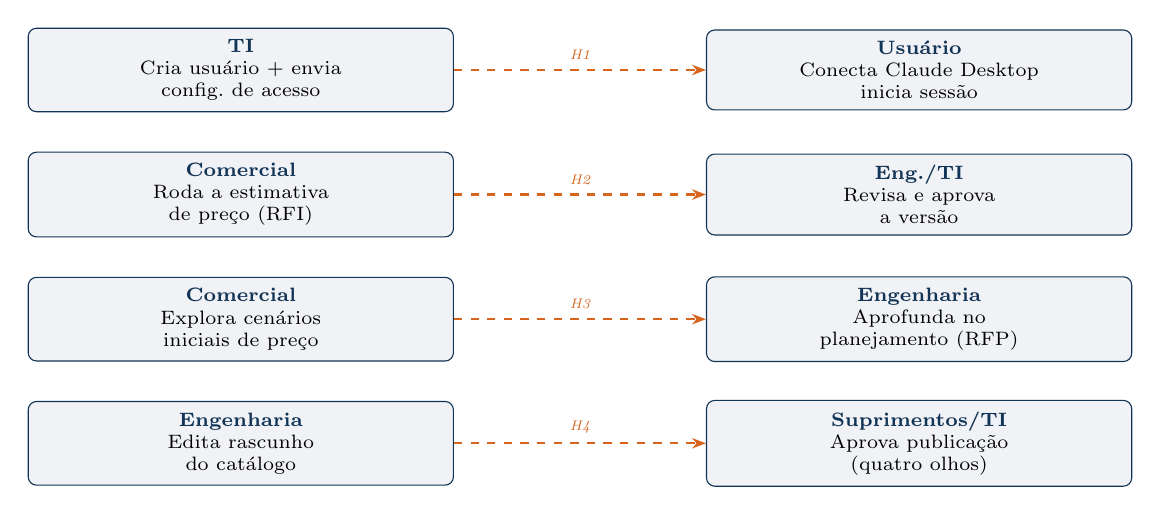
\begin{tikzpicture}[
      handoff/.style={draw=mlblue,fill=mlgray,rounded corners=3pt,
                   minimum width=5.4cm,minimum height=0.85cm,
                   font=\scriptsize,align=center,inner sep=4pt},
      hoff/.style={-{Stealth[length=5pt]},mlorange,thick,dashed},
    ]
    % H1
    \node[handoff] (ti1)
      {\textbf{\textcolor{mlblue}{TI}}\\Cria usuário + envia\\config.\ de acesso};
    \node[handoff,right=3.2cm of ti1] (op1)
      {\textbf{\textcolor{mlblue}{Usuário}}\\Conecta Claude Desktop\\inicia sessão};
    \draw[hoff] (ti1) -- node[above,font=\tiny\itshape,mlorange]{H1} (op1);

    % H2
    \node[handoff,below=0.5cm of ti1] (op2)
      {\textbf{\textcolor{mlblue}{Comercial}}\\Roda a estimativa\\de preço (RFI)};
    \node[handoff,right=3.2cm of op2] (en2)
      {\textbf{\textcolor{mlblue}{Eng./TI}}\\Revisa e aprova\\a versão};
    \draw[hoff] (op2) -- node[above,font=\tiny\itshape,mlorange]{H2} (en2);

    % H3
    \node[handoff,below=0.5cm of op2] (op3)
      {\textbf{\textcolor{mlblue}{Comercial}}\\Explora cenários\\iniciais de preço};
    \node[handoff,right=3.2cm of op3] (en3)
      {\textbf{\textcolor{mlblue}{Engenharia}}\\Aprofunda no\\planejamento (RFP)};
    \draw[hoff] (op3) -- node[above,font=\tiny\itshape,mlorange]{H3} (en3);

    % H4
    \node[handoff,below=0.5cm of op3] (en4)
      {\textbf{\textcolor{mlblue}{Engenharia}}\\Edita rascunho\\do catálogo};
    \node[handoff,right=3.2cm of en4] (su4)
      {\textbf{\textcolor{mlblue}{Suprimentos/TI}}\\Aprova publicação\\(quatro olhos)};
    \draw[hoff] (en4) -- node[above,font=\tiny\itshape,mlorange]{H4} (su4);
  \end{tikzpicture}
  \vspace{2pt}

  {\scriptsize
    \textbf{H1} Onboarding de usuário \quad
    \textbf{H2} Execução $\to$ aprovação \\
    \textbf{H3} Estimativa $\to$ planejamento \quad
    \textbf{H4} Atualização de catálogo
  }
\end{frame}

% ═══════════════════════════════════════════════════════════════════════════
\section{Encerramento}
% ═══════════════════════════════════════════════════════════════════════════

\subsection{Síntese e próximos passos}
\begin{frame}
  \mtitle{Síntese e Próximos Passos}
  \begin{columns}[T]
    \column{0.5\textwidth}
    \begin{block}{O que levar desta apresentação}
      \begin{enumerate}\small
        \item \textbf{Trilha auditável} do salário ao preço de venda ---
          e preços \emph{concluídos} por composição, não digitados
        \item \textbf{Tempo e recursos otimizados juntos}: RCPSP + pool
          de equipes + estoque de materiais
        \item \textbf{Governança por construção}: quatro olhos,
          versionamento e papéis --- não por procedimento em papel
      \end{enumerate}
    \end{block}
    \column{0.46\textwidth}
    \begin{block}{Próximos passos}
      \begin{itemize}\scriptsize
        \item Recotações sinalizadas no próprio catálogo
          (alertas de preço defasado já gravados no dado)
        \item Piloto produtor-consumidor com dados de campo
          (confirmar capacidade real da obra)
      \end{itemize}
    \end{block}
    \vspace{6pt}
    \begin{exampleblock}{}
      \centering\large Perguntas?
    \end{exampleblock}
  \end{columns}
\end{frame}


% ═══════════════════════════════════════════════════════════════════════════
\appendix
\section{Apêndice}
% ═══════════════════════════════════════════════════════════════════════════

\subsection{Fluxo de entrega}
\begin{frame}
  \frametitle{\textcolor{mlorange}{A.1}\quad Processo de Deploy: Blue-Green no Azure ACA}
  \begin{block}{Etapas}
    \centering
    \resizebox{\linewidth}{!}{%
    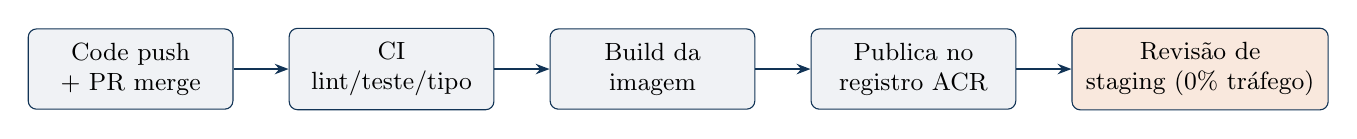
\begin{tikzpicture}[
        box/.style={draw=mlblue,fill=mlgray,rounded corners=3pt,font=\small,
                    align=center,inner sep=5pt,minimum width=2.6cm,minimum height=0.9cm},
        arr2/.style={-{Stealth[length=5pt]},mlblue,thick},
      ]
      \node[box] (b1) {Code push\\+ PR merge};
      \node[box,right=0.7cm of b1] (b2) {CI\\lint/teste/tipo};
      \node[box,right=0.7cm of b2] (b3) {Build da\\imagem};
      \node[box,right=0.7cm of b3] (b4) {Publica no\\registro ACR};
      \node[box,right=0.7cm of b4,fill=mlorange!15] (b5) {Revisão de\\staging (0\% tráfego)};
      \draw[arr2] (b1) -- (b2);
      \draw[arr2] (b2) -- (b3);
      \draw[arr2] (b3) -- (b4);
      \draw[arr2] (b4) -- (b5);
    \end{tikzpicture}}
  \end{block}
  \vspace{-4pt}
  \begin{center}
    \tikz{\draw[-{Stealth[length=5pt]},mlblue,thick] (0,0.22) -- (0,-0.02);}
    {\tiny\itshape roda contra a revisão de staging (0\% tráfego)}
  \end{center}
  \vspace{-6pt}
  \begin{block}{Smoke test --- 15 verificações automáticas}
    \tiny
    \begin{columns}[T]
      \column{0.5\textwidth}
      \yes\ Saúde do sistema \\
      \yes\ Emissão de token \\
      \yes\ Rejeita acesso sem token (401) \\
      \yes\ Rate limit no /auth/token (429) \\
      \yes\ Token contém claim `roles' \\
      \yes\ Token contém claim `sub' \\
      \yes\ Leitura de projetos com token válido \\
      \column{0.5\textwidth}
      \yes\ Headers de rate limit presentes \\
      \yes\ RBAC nega endpoint restrito (403) \\
      \yes\ Leitura do catálogo \\
      \yes\ Servidor MCP responde \\
      \yes\ MCP tools/list com token \\
      \yes\ MCP rejeita sem token (401) \\
      \yes\ Certificado TLS válido \quad \yes\ HTTPS redirect \\
    \end{columns}
    \vspace{1pt}
    {\tiny\itshape 9 dessas verificações exigem credencial de smoke test configurada.}
  \end{block}
  \vspace{-4pt}
  \centering{\tiny\itshape resultado do smoke test}\par
  \vspace{-3pt}
  \begin{columns}[T]
    \column{0.48\textwidth}
    \centering\tikz{\draw[-{Stealth[length=5pt]},mlred,thick] (0,0.2) -- (0,-0.02);}
    \column{0.48\textwidth}
    \centering\tikz{\draw[-{Stealth[length=5pt]},mlgreen,thick] (0,0.2) -- (0,-0.02);}
  \end{columns}
  \vspace{-8pt}
  \begin{columns}[T]
    \column{0.48\textwidth}
    \begin{alertblock}{\small Falhou}
      \scriptsize Rollback. Revisão de staging permanece em 0\%; 100\% do
      tráfego segue na revisão atual.
    \end{alertblock}
    \column{0.48\textwidth}
    \begin{exampleblock}{\small Passou}
      \scriptsize Promove tráfego: nova revisão 0\%$\to$100\%; revisão
      anterior desmobilizada.
    \end{exampleblock}
  \end{columns}
\end{frame}

\subsection{Ferramentas MCP por grupo}
\begin{frame}
  \frametitle{\textcolor{mlorange}{A.2}\quad Referência: Ferramentas MCP por Grupo.Ação (47 no total)}
  \begin{columns}[T]
    \column{0.5\textwidth}
    \begin{block}{\tiny Sistema (1)}
      \tiny\texttt{ping}
    \end{block}
    \vspace{1pt}
    \begin{block}{\tiny Projetos (25)}
      \tiny
      \textbf{Leitura (11)}:
      \texttt{listar\_projetos, consultar\_status,
      consultar\_estrutura\_projeto, consultar\_job\_pipeline,
      listar\_jobs\_pipeline, comparar\_planos, explorar\_pool\_recursos,
      explorar\_estoque\_consumiveis, auditar\_plano, consultar\_benchmark,
      listar\_runs\_campanha}\\[3pt]
      \textbf{Criação e execução (10)}:
      \texttt{criar\_projeto, iniciar\_orcamento, nova\_versao,
      gerir\_escopo, disparar\_pipeline, cancelar\_job\_pipeline,
      salvar\_perfil\_bdi, simular\_cenario\_replan, empacotar\_benchmark,
      explorar\_configuracoes\_go}\\[3pt]
      \textbf{Aprovação (1)}: \texttt{aprovar\_versao}\\[3pt]
      \textbf{Artefatos (3)}:
      \texttt{listar\_artefatos\_projeto, obter\_artefato,
      download\_benchmark\_zip}
    \end{block}
    \column{0.5\textwidth}
    \begin{block}{\tiny\textcolor{mlteal}{Catálogo} (15)}
      \tiny
      \textbf{Leitura (10)}:
      \texttt{listar\_contextos, pesquisar\_catalogo,
      auditar\_catalogo, historico\_preco\_insumo, calcular\_pu\_producao,
      versoes\_catalogo, listar\_divergencias\_rascunho,
      consultar\_impacto\_reajuste, exportar\_pesquisa\_mercado,
      calcular\_tributos}\\[3pt]
      \textbf{Escrita e merge (5)}:
      \texttt{atualizar\_preco\_insumo, adicionar\_variante\_producao,
      criar\_rascunho\_catalogo, aprovar\_merge\_catalogo (4 olhos),
      rejeitar\_rascunho\_catalogo}
    \end{block}
    \vspace{1pt}
    \begin{block}{\tiny\textcolor{mlgreen}{Financeiro} (2)}
      \tiny\texttt{comparar\_rfi\_catalogo, obter\_resultado\_campanha}
    \end{block}
    \vspace{1pt}
    \begin{block}{\tiny\textcolor{mlpurple}{Autenticação / dispositivos} (4)}
      \tiny\texttt{ativar\_dispositivo, renovar\_token,
      listar\_meus\_dispositivos, revogar\_meu\_dispositivo}
    \end{block}
  \end{columns}
  \vspace{1pt}
  {\tiny\itshape Fonte: introspecção de \texttt{build\_server()} + tags
  \texttt{@permission} --- Autenticação/dispositivos é auto-serviço de token,
  fora das 8 categorias do slide 3.2.}
\end{frame}


\end{document}
